\chapter{À la recherche de la généralisation de l'arbre minimum couvrant}
\label{chap:generalisation_mst}

Au cours du chapitre \ref{chap:hgp_clusterer} précédent, nous avons montré que les $K$-polyèdres de \v Cech constituent la bonne généralisation du Single-Linkage : niveau par niveau, la hiérarchie qu'ils produisent coïncide avec les amas discrets de forte densité de l'estimateur \KNN (\Th[th:cech_kpolyedres_knn]).
Cette réponse est satisfaisante mathématiquement, mais quelque peu brutale algorithmiquement. Construire le complexe de \v Cech complet revient à manipuler tous les $K$-simplexes sur $\mathcal X$, au nombre de $\binom n{K+1}$.

Pour $K=1$, cette explosion n'a pas lieu en pratique dans l'espace euclidien (de petite dimension) : on ne calcule pas toute la filtration des graphes géométriques, on extrait l'arbre minimum couvrant. %Le \Th~\ref{th:mst_gg} affirme alors que l'arbre minimum couvrant élagué à l'échelle $r$ possède exactement les mêmes composantes connexes que le graphe géométrique de rayon $r$. 
Cet arbre est lui-même contenu dans le graphe de \nom{Gabriel}, lui-même sous-graphe de la triangulation de \nom{Delaunay} (\Res[res:MSTsous-graphe]).

L'objectif de ce chapitre est de reconstruire cette chaîne d'idées à l'ordre $K$ :
\begin{multline*}
    \text{Complexes de \v Cech} 
    \quad\leadsto\quad \text{Simplexes responsables des fusions} \\
    \quad\leadsto\quad \text{$K$-Graphe de \nom{Gabriel}}
    \quad\leadsto\quad \text{Mosaïque de \nom{Delaunay} d'ordre }K
\end{multline*}

%Le point délicat est que, pour $K\ge2$, un simplexe ne relie plus seulement deux sommets : un $K$-simplexe recolle simultanément ses $K+1$ facettes de dimension $K-1$. Il faut donc prendre au sérieux la structure combinatoire portée par les facettes, et non plus seulement par les points.

\Contributions{Ce chapitre reprend et développe les optimisations géométriques introduites dans \cite{BibiAppliedNetworkScience}. Nous commençons par montrer que l'on peut retrouver les $K$-polyèdres comme composantes connexes d'un graphe pondéré \emph{élémentaire} sur les $(K-1)$-simplexes, c'est-à-dire en restreignant les arêtes aux $K$-simplexes. Cette reformulation permet de définir précisément les simplexes $K$-séparants (\Def[def:chapIV_simplexe_separant]) : les simplexes qui provoquent effectivement une fusion dans la hiérarchie. Le premier résultat central est le \Th~\ref{th:chapIV_separant_gabriel} : tout simplexe $K$-séparant est nécessairement de \nom{Gabriel}. On en déduit que le graphe de \nom{Gabriel} contient toutes les fusions utiles et qu'un arbre couvrant minimum construit sur ce graphe préserve, à chaque échelle, les $K$-polyèdres (\Th[th:chapIV_cech_kmst]). Enfin, nous expliquons comment construire en pratique la hiérarchie \KNN : la structure géométrique naturelle derrière cette construction est la mosaïque de \nom{Delaunay} d'ordre $K$.}

\section{L'approche persistante : les simplexes $K$-\emph{séparants}}
\label{sec:chapIV_simplexes_separants}

Fixons un nuage fini $\mathcal X\subset\mathbb R^p$ et un entier
\[
    K\in\IntervalleEntiers{1,|\mathcal X|-1}.
\]
%Dans tout ce chapitre, un $k$-simplexe est identifié à un sous-ensemble de $\mathcal X$ de cardinal $k+1$.

\begin{Definition}{Rayon de naissance d'un simplexe}{chapIV_rayon_naissance}
Pour tout sous-ensemble fini non vide $\sigma\subseteq\mathcal X$, on note
\[
\boxed{
    \rho(\sigma)
    \eqdef
    \inf\left\{r\ge0 \mid \sigma\in\check C(\mathcal X,r)\right\}.
    }
\]
Autrement dit,
\[
    \rho(\sigma)
    =
    \inf_{y\in\mathbb R^p}\max_{x\in\sigma}\norme{y-x}.
\]
La boule fermée réalisant cet infimum sera notée
\[
\boxed{
    B_\sigma = \overline B(c_\sigma,\rho(\sigma)),
    }
\]
avec $c_\sigma$ son centre. 
\end{Definition}
\Remarque{En anglais, on appelle cette plus petite boule englobante la \emph{miniball} de $\sigma$. La méthode standard pour calculer le rayon $\rho(\sigma)$ ainsi que pour identifier le centre $c_\sigma$ de la boule $B_\sigma$ est l'algorithme de \nom{Welzl} \cite{Welzl1991}.}

%Ainsi $\rho(\sigma)$ est le rayon de la plus petite boule fermée contenant les sommets de $\sigma$. 
Le rayon de naissance $\rho(\sigma)$ est exactement le niveau d'apparition de $\sigma$ dans la filtration de \v Cech. Pour $K=1$, si $\sigma=\{x,x'\}$, alors
\[
    \rho(\sigma)=\frac12\norme{x-x'}.
\]

Dans toute la suite du chapitre, nous utiliserons l'hypothèse suivante à propos des données $\mathcal X$. %Elle n'est pas conceptuellement essentielle ; elle évite seulement les discussions sur les égalités simultanées de rayons et les points cosphériques.

\begin{Definition}{Position générale pour la filtration de \v Cech}{chapIV_position_generale_cech}
On dit qu'un nuage $\mathcal X\subset \mathbb R^p$ localement fini est en \emph{position générale pour la filtration de \v Cech} si, pour tout simplexe $\sigma\subseteq\mathcal X$ avec $\module{\sigma} \ge 2$,
% \begin{enumerate}
%     \item 
aucun point de $\mathcal X\setminus\sigma$ n'appartient à la frontière de sa plus petite boule englobante,
    \[
        \partial B_\sigma\cap(\mathcal X\setminus\sigma)=\varnothing.
    \]
%     \item Les points de $\sigma\cap\partial B_\sigma$ sont affinement indépendants et $c_\sigma$ appartient à l'intérieur (relatif) de leur enveloppe convexe.
% \end{enumerate}
% En particulier, les points de $\sigma\cap\partial B_\sigma$ forment l'ensemble de support de la boule minimale.
Autrement dit, aucun point du nuage extérieur à $\sigma$ ne se trouve sur
la frontière de la plus petite boule englobante de $\sigma$.
\end{Definition}

\Remarques{
\begin{enumerate}
    \item Noter que notre définition d'un nuage en position générale est plus contraignante que la \Def~4.2 de \cite{BoissonnatChazalYvinec}
    \item Sous cette hypothèse, les points de $\sigma\cap\partial B_\sigma$ forment
exactement l'ensemble de support de la boule minimale $B_\sigma$  (voir \Res~\ref{res:chapIV_miniball_support} ci-dessous).
En particulier, ils sont affinement indépendants et $c_\sigma$ appartient à l'intérieur (relatif) de 
$
\operatorname{conv}(\sigma\cap\partial B_\sigma).
$
\end{enumerate}
}

\begin{Resultat}{Boule minimale et ensemble de support \cite{Welzl1991, BoissonnatChazalYvinec}}{chapIV_miniball_support}
Soit $A\subset\mathbb R^p$ fini non vide. Il existe une unique plus petite boule fermée contenant $A$. Son centre appartient à l'enveloppe convexe d'un sous-ensemble
\[
    S(A)\subseteq A\cap\partial B_A
\]
de cardinal au plus $p+1$. Sous l'hypothèse de position générale (\Def~\ref{def:chapIV_position_generale_cech}), cet ensemble de support est exactement l'ensemble des points de $A$ situés sur la frontière de $B_A$. En particulier, si $s\in S(A)$, alors
\[
\boxed{
    \rho(A\setminus\{s\})<\rho(A).
    }
\]
\end{Resultat}

\begin{figure}[!h]
    \centering
    % ---------- SOUS-FIGURE A : Triangle acutangle ----------
    \begin{subfigure}[b]{0.48\textwidth}
        \centering
        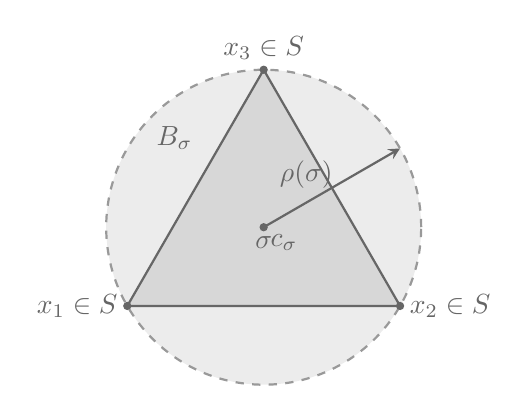
\begin{tikzpicture}[scale=1.]
            % Coordonnées
            \coordinate (C) at (0,0);
            
            % Boule minimale B_sigma
            \fill[gray!15] (C) circle (2);
            \draw[dashed, gray!80, thick] (C) circle (2);
            \node[gray!80!black] at (135:1.6) {$B_\sigma$};

            % Sommets du simplexe (tous sur la frontière)
            \coordinate (X1) at (210:2);
            \coordinate (X2) at (330:2);
            \coordinate (X3) at (90:2);

            % Simplexe sigma
            \fill[gray!35, fill opacity=0.8] (X1) -- (X2) -- (X3) -- cycle;
            \draw[thick, gray!80!black] (X1) -- (X2) -- (X3) -- cycle;
            \node[gray!80!black] at (0, -0.2) {$\sigma$};

            % Centre c_sigma et rayon rho(sigma)
            \draw[->, >=stealth, gray!80!black, thick] (C) -- (30:2) node[midway, above left=-4pt] {$\rho(\sigma)$};
            \fill[gray!80!black] (C) circle (1.5pt) node[below right=-1pt] {$c_\sigma$};

            % Sommets et appartenance à S
            \fill[gray!80!black] (X1) circle (1.5pt) node[left] {$x_1 \in S$};
            \fill[gray!80!black] (X2) circle (1.5pt) node[right] {$x_2 \in S$};
            \fill[gray!80!black] (X3) circle (1.5pt) node[above] {$x_3 \in S$};
        \end{tikzpicture}
        \caption{\textbf{Triangle aigu.} Le centre $c_\sigma$ se trouve à l'intérieur de l'enveloppe convexe. Tous les sommets définissent la boule minimale, donc $S = \sigma$.}
        \label{fig:support_acutangle}
    \end{subfigure}
    \hfill
    % ---------- SOUS-FIGURE B : Triangle obtusangle ----------
    \begin{subfigure}[b]{0.48\textwidth}
        \centering
        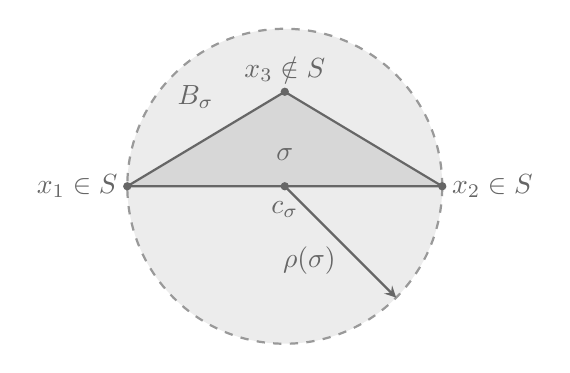
\begin{tikzpicture}[scale=1.]
            % Coordonnées
            \coordinate (C) at (0,0);
            
            % Boule minimale B_sigma
            \fill[gray!15] (C) circle (2);
            \draw[dashed, gray!80, thick] (C) circle (2);
            \node[gray!80!black] at (135:1.6) {$B_\sigma$};

            % Sommets du simplexe (2 sur la frontière, 1 à l'intérieur)
            \coordinate (X1) at (180:2);
            \coordinate (X2) at (0:2);
            \coordinate (X3) at (0,1.2);

            % Simplexe sigma
            \fill[gray!35, fill opacity=0.8] (X1) -- (X2) -- (X3) -- cycle;
            \draw[thick, gray!80!black] (X1) -- (X2) -- (X3) -- cycle;
            \node[gray!80!black] at (0, 0.4) {$\sigma$};

            % Centre c_sigma et rayon rho(sigma)
            \draw[->, >=stealth, gray!80!black, thick] (C) -- (-45:2) node[midway, below left=-2pt] {$\rho(\sigma)$};
            \fill[gray!80!black] (C) circle (1.5pt) node[below=2pt] {$c_\sigma$};

            % Sommets et appartenance à S
            \fill[gray!80!black] (X1) circle (1.5pt) node[left] {$x_1 \in S$};
            \fill[gray!80!black] (X2) circle (1.5pt) node[right] {$x_2 \in S$};
            \fill[gray!80!black] (X3) circle (1.5pt) node[above] {$x_3 \notin S$};
        \end{tikzpicture}
        \caption{Triangle obtus : le centre $c_\sigma$ appartient à une arête. L'ensemble de support est strictement inclus dans le simplexe : $S = \{x_1,x_2\} \subsetneq \sigma$.}
        \label{fig:support_obtusangle}
    \end{subfigure}
    \caption{Illustration de la plus petite boule englobante $B_\sigma$, de son centre $c_\sigma$, de son rayon de naissance $\rho(\sigma)$ et de son ensemble de support à la frontière $S = \sigma \cap \partial B_\sigma$ pour un $2$-simplexe $\sigma=\{x_1,x_2,x_3\}$.}
    \label{fig:illustrations_definitions_simplexe}
\end{figure}


\subsection{Le graphe élémentaire des facettes}

Il nous a été plus commode en \Def[def:k_polyedres] de définir les $K$-polyèdres comme les composantes connexes d'un graphe $\Gamma_K(\mathcal X,r)$ dont les sommets sont les $(K-1)$-simplexes de $\check C(\mathcal X,r)$ et dont deux sommets sont adjacents lorsque leur union est encore un simplexe de $\check C(\mathcal X,r)$, et ce sans restriction sur la taille de cette union. 
L'objet de \Fact~\ref{fait:chapIV_adjacences_elementaires} est d'observer que l'on aurait pu se restreindre aux adjacences \emph{élémentaires}, c'est-à-dire aux seuls $K$-simplexes pour créer des liaisons entre les sommets.


% Un $K$-simplexe $\sigma$ induit donc une clique de taille $K+1$ sur l'ensemble de ses facettes
% \[
%     \mathcal F(\sigma)
%     \eqdef
%     \{\sigma\setminus\{x\}:x\in\sigma\},
% \]
% et toutes les arêtes de cette clique portent le même poids $\rho(\sigma)$.

\begin{Fait}{Les adjacences élémentaires suffisent}{chapIV_adjacences_elementaires}
Pour tout $r\ge0$, retirer de $\Gamma_K(\mathcal X,r)$ les liens entre deux sommets  $\tau$ et $\tau'$ dès que $\module{\tau \cup \tau'} > K+1$ laisse inchangées les composantes connexes. Elles correspondent donc toujours aux $K$-polyèdres du complexe de \v Cech $\check C(\mathcal X,r)$ définis en \Def~\ref{def:k_polyedres}.
\end{Fait}

\begin{Preuve}
Supposons que deux $(K-1)$-simplexes $\tau$ et $\tau'$ soient adjacents dans $\Gamma_K(\mathcal X,r)$, c'est-à-dire que $\tau \cup \tau' \in\check C(\mathcal X,r)$, soit
\[
    \rho(\tau\cup\tau') \le r .
\]
Si $|\tau \cup \tau'|=K+1$, l'adjacence est déjà élémentaire. Si $|\tau \cup \tau'|>K+1$, alors on peut relier $\tau$ à $\tau'$ au moyen d'un chemin de $K$-sous-simplexes de $\tau \cup \tau'$, différant à chaque fois d'un seul élément. Ces liaisons sont toutes présentes dans le graphe $\Gamma_K(\mathcal X,r)$ élagué des simplexes de dimension $>K$.
\end{Preuve}

\Notation{À partir de maintenant,  $\Gamma_K(\mathcal X,r)$ désignera uniquement la version élaguée du graphe, réduit aux adjacences élémentaires. Nous noterons ce graphe indifféremment $\Gamma_K(\mathcal X)_{\le r}$ et $\Gamma_K(\mathcal X)$, sans indice, quand nous prenons $r=+\infty$. Nous noterons aussi $\Gamma_K(\mathcal X)_{< r}$ le sous-graphe de $\Gamma_K(\mathcal X)_{\le r}$ privé de tous les simplexes $\sigma$ (sommets et arêtes) ayant un rayon $\rho(\sigma)$ exactement égal à $r$.}

\begin{Definition}{Simplexe $K$-séparant}{chapIV_simplexe_separant}
Soit $\sigma\subseteq\mathcal X$ un $K$-simplexe, et posons
\[
    r_\sigma \eqdef \rho(\sigma).
\]
On appelle \emph{facettes actives} de $\sigma$ les facettes déjà présentes strictement avant la naissance de $\sigma$ :
\[
    \mathcal F_{<}(\sigma)
    \eqdef
    \left\{
        \tau\subset\sigma
        \ \middle|\
        \module{\tau}=K
        \ \text{et}\
        \rho(\tau)<r_\sigma
    \right\}.
\]
On dit que $\sigma$ est \emph{$K$-séparant} s'il existe deux facettes actives
\[
    \tau,\tau'\in\mathcal F_{<}(\sigma)
\]
qui appartiennent à deux composantes connexes distinctes de
\[
    \Gamma_K(\mathcal X)_{<r_\sigma}.
\]
Autrement dit, $\sigma$ est $K$-séparant lorsqu'il provoque effectivement une fusion entre deux $K$-polyèdres déjà présents.
\end{Definition}

\Remarque{
Sous l'hypothèse de position générale pour la filtration de \v Cech, un $K$-simplexe $\sigma$ possède toujours au moins deux facettes actives. En effet, si
\[
    S_\sigma \eqdef \sigma\cap\partial B_\sigma
\]
désigne l'ensemble de support de sa plus petite boule englobante, alors $\module{S_\sigma}\ge2$ et, pour tout $s\in S_\sigma$,
\[
    \rho(\sigma\setminus\{s\})<\rho(\sigma).
\]
Les facettes actives sont donc au moins les $\sigma\setminus\{s\}$, avec $s\in S_\sigma$. Les autres facettes, obtenues en retirant un sommet intérieur de $B_\sigma$, peuvent en revanche naître exactement au même niveau que $\sigma$.
}

Autrement dit, un simplexe $K$-séparant est un simplexe qui change réellement la connectivité persistante des $K$-polyèdres. Pour $K=1$, les $1$-simplexes séparants sont exactement les arêtes qui relient deux composantes distinctes du graphe géométrique au moment où elles apparaissent ; ce sont les arêtes de l'arbre minimum couvrant.

Le \Res~\ref{res:chapIV_mst_sous_niveaux_graphe} appliqué à $\Gamma_K(\mathcal X)$ dit que si l'on savait construire un arbre couvrant minimum de $\Gamma_K(\mathcal X)$, alors son élagage à l'échelle $r$ redonnerait les $K$-polyèdres de $\check C(\mathcal X,r)$. Mais ce graphe contient encore tous les sommets induits par les $\binom n{K}$ simplexes d'ordre $K-1$. Il faut donc identifier un sous-graphe beaucoup plus mince ; c'est l'objet de la section suivante.

\section{Une condition nécessaire pour un simplexe séparant : être de \nom{Gabriel}}
\label{sec:chapIV_k_gabriel}

Le cas $K=1$ fournit l'intuition géométrique décisive : une arête de l'arbre minimum couvrant euclidien est nécessairement une arête de \nom{Gabriel} (\Def~\ref{def:gabriel} \& \Res[res:MSTsous-graphe]), c'est-à-dire que la plus petite boule englobante, celle ayant pour diamètre l'arête, est vide de tout autre point du nuage. La condition se généralise en remplaçant la boule diamétrale par la plus petite boule englobante du simplexe.

\begin{Definition}{Simplexe de \nom{Gabriel}}{chapIV_k_gabriel_simplex}
Un $K$-simplexe $\sigma\subseteq\mathcal X$ est dit de \emph{\nom{Gabriel}} si l'intérieur de sa plus petite boule englobante ne contient aucun point de $\mathcal X$ extérieur à $\sigma$ :
\[
\boxed{
    \mathring{B}_\sigma\cap(\mathcal X\setminus\sigma)=\varnothing.
    }
\]
\end{Definition}

\Remarque{Noter que notre généralisation de la notion de simplexe de \nom{Gabriel} à l'aide de la \emph{miniball} diffère de celle de \cite{BoissonnatChazalYvinec}, où l'on impose une condition de sphère circonscrite vide (la \emph{circumball}). Pour $K=1$, les deux notions coïncident avec l'arête de \nom{Gabriel} classique.
%Pour $K=2$, elles diffèrent exactement sur les triangles obtus : la boule minimale est alors le disque de diamètre le plus long côté, et non le cercle circonscrit.
}

Cette condition de vacuité est nécessaire pour qu'un $K$-simplexe provoque une fusion.

\begin{Theoreme}{Condition nécessaire pour que $\sigma$ soit $K$-séparant : $\sigma$ doit être de \nom{Gabriel}}{chapIV_separant_gabriel}
Supposons $\mathcal X$ en position générale pour la filtration de \v Cech. Tout simplexe $K$-séparant est de \nom{Gabriel}.
\end{Theoreme}

\begin{Preuve}[{Preuve du \Th~\ref{th:chapIV_separant_gabriel}}]
Soit $\sigma$ un $K$-simplexe, et posons
\[
    r=\rho(\sigma),
    \qquad
    B_\sigma=\overline B(c,r).
\]
Raisonnons par contraposée. Supposons que $\sigma$ ne soit pas de \nom{Gabriel}. Il existe donc un point
\[
    z\in \mathcal X\setminus\sigma
    \qquad\text{tel que}\qquad
    z\in\mathring{B}_\sigma.
\]
Notons
\[
    S\eqdef \sigma\cap\partial B_\sigma
\]
l'ensemble des sommets de $\sigma$ situés sur la frontière de la boule minimale. Par la \Def~\ref{def:chapIV_position_generale_cech} et le \Res~\ref{res:chapIV_miniball_support}, $S$ est l'ensemble de support de $B_\sigma$ ; en particulier $|S|\ge2$, le centre $c$ appartient à l'intérieur relatif de $\operatorname{conv}(S)$, et retirer n'importe quel point de $S$ diminue strictement le rayon de naissance.

% \begin{figure}[!h]
%     \centering
%     % ---------- SOUS-FIGURE A : L'hypothèse de départ (Triangle obtus) ----------
%     \begin{subfigure}[b]{0.48\textwidth}
%         \centering
%         \begin{tikzpicture}[scale=1.2]
%             % Coordonnées
%             \coordinate (C) at (0,0);
%             \coordinate (S) at (-2,0);
%             \coordinate (T) at (2,0);
%             \coordinate (U) at (0,1);
%             \coordinate (Z) at (0,-1);

%             % Boule minimale B_sigma (Cercle diamétral de [s,t])
%             \fill[gray!10] (C) circle (2);
%             \draw[dashed, gray!80, thick] (C) circle (2);
%             \node[gray!80!black] at (135:1.6) {$B_\sigma$};

%             % Simplexe sigma (Triangle obtus)
%             \fill[blue!10, fill opacity=0.8] (S) -- (T) -- (U) -- cycle;
%             \draw[thick, blue!80!black] (S) -- (T) -- (U) -- cycle;
%             \node[blue!80!black] at (0, 0.35) {$\sigma$};

%             % Centre c et rayon r
%             \draw[->, >=stealth, gray!80!black, thick] (C) -- (-30:2) node[midway, below=1pt] {$r$};
%             \fill (C) circle (1.5pt) node[above right=-2pt] {$c$};

%             % Sommets s, t (Points de support) et u (intérieur)
%             \fill (S) circle (1.5pt) node[left] {$s \in S$};
%             \fill (T) circle (1.5pt) node[right] {$t \in S$};
%             \fill (U) circle (1.5pt) node[above] {$u \notin S$};
            
%             % Point intrus z
%             \fill[red] (Z) circle (2pt) node[below right=-1pt, red] {$z$};

%         \end{tikzpicture}
%         \caption{Un triangle $\sigma=\{s,t,u\}$. $B_\sigma$ a pour diamètre $[s,t]$. L'ensemble de support est $S=\{s,t\}$. $\sigma$ n'est pas de \nom{Gabriel} donc il existe un ``intrus'' $z \in \mathring{B}_\sigma$.}
%         \label{fig:thm6_a}
%     \end{subfigure}
%     \hfill
%     % ---------- SOUS-FIGURE B : Le chemin de contournement ----------
%     \begin{subfigure}[b]{0.48\textwidth}
%         \centering
%         \begin{tikzpicture}[scale=1.2]
%             % Coordonnées
%             \coordinate (C) at (0,0);
%             \coordinate (S) at (-2,0);
%             \coordinate (T) at (2,0);
%             \coordinate (U) at (0,1);
%             \coordinate (Z) at (0,-1);

%             % Centres et rayon des nouvelles boules minimales
%             % Par calcul exact géométrique : le rayon est de 1.25 et les centres sont à (+/- 0.75, 0)
%             \coordinate (Ct) at (-0.75, 0);
%             \coordinate (Cs) at (0.75, 0);
%             \def\Rnew{1.25}

%             % Boule originale en filigrane (repère visuel)
%             \draw[dotted, gray!60, thick] (C) circle (2);
            
%             % L'arête non-active tau_u={s,t} est grisée pour montrer qu'elle n'est pas dans le chemin
%             \draw[thick, gray!40] (S) -- (T);

%             % Boules minimales des simplexes alternatifs
%             \fill[red!10, fill opacity=0.5] (Ct) circle (\Rnew);
%             \draw[dashed, red!80!black, thick] (Ct) circle (\Rnew);

%             \fill[green!10, fill opacity=0.5] (Cs) circle (\Rnew);
%             \draw[dashed, green!80!black, thick] (Cs) circle (\Rnew);

%             % Simplexes alternatifs construits avec z
%             \fill[red!20, fill opacity=0.6] (S) -- (U) -- (Z) -- cycle;
%             \draw[thick, red!80!black] (S) -- (U) -- (Z) -- cycle;

%             \fill[green!20, fill opacity=0.6] (T) -- (U) -- (Z) -- cycle;
%             \draw[thick, green!80!black] (T) -- (U) -- (Z) -- cycle;

%             % Chemin des facettes actives (en gras pour bien le faire ressortir)
%             \draw[line width=1.5pt, red!80!black] (S) -- (U) node[midway, above left=-2pt] {$\tau_t$};
%             \draw[line width=1.5pt, green!80!black] (T) -- (U) node[midway, above right=-2pt] {$\tau_s$};
%             \draw[line width=1.5pt, purple] (U) -- (Z) node[midway, right=1pt] {$\eta_{s,t}^z$};

%             % Sommets et intrus
%             \fill (S) circle (1.5pt) node[left] {$s$};
%             \fill (T) circle (1.5pt) node[right] {$t$};
%             \fill (U) circle (1.5pt) node[above] {$u$};
%             \fill[purple] (Z) circle (2pt) node[below right=-1pt] {$z$};

%             % Étiquettes des simplexes
%             \node[red!80!black] at (-1.1, -0.3) {$\sigma_t^z$};
%             \node[green!80!black] at (1.1, -0.3) {$\sigma_s^z$};
            
%         \end{tikzpicture}
%         \caption{Les $K$-simplexes $\sigma_t^z$ et $\sigma_s^z$ ont des rayons $ < r$. Le chemin $\tau_s \xleftrightarrow{\sigma_s^z}_r \eta_{s,t}^z \xleftrightarrow{\sigma_t^z}_r \tau_t$ connecte les facettes actives dans $\Gamma_K(\mathcal{X})_{<r}$. %Ainsi, il n'y a pas de changement des $2$-polyèdres de $\Gamma_2(\mathcal{X})_{\le r}$.
%         }
%         \label{fig:thm6_b}
%     \end{subfigure}
%     \caption{Illustration de la preuve du \Th~\ref{th:chapIV_separant_gabriel} ($K=2$) pour un triangle $\sigma=\{s,t,u\}$ obtus en $u$, c'est-à-dire que $S = \{s,t\}$. Si le simplexe n'est pas de \nom{Gabriel}, $B_\sigma$ (de rayon $r$) contient donc un ``intrus'' $z$. Les facettes $\tau_s$ et $\tau_t$, actives pour une filtration $<r$, sont connectées au moyen de $z$ (les $2$-simplexes $\sigma_s^z$ et $\sigma_t^z$)}
%     \label{fig:preuve_gabriel_obtus}
% \end{figure}

\begin{figure}[!h]
    \centering
    % ---------- SOUS-FIGURE A : L'hypothèse de départ (Triangle obtus) ----------
    \begin{subfigure}[b]{0.48\textwidth}
        \centering
        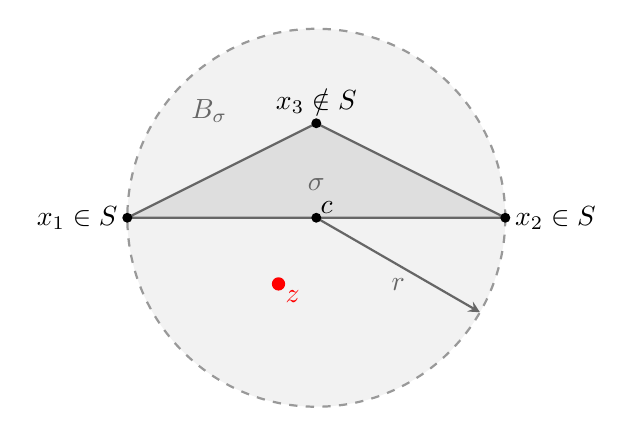
\begin{tikzpicture}[scale=1.2]
            % Coordonnées
            \coordinate (C) at (0,0);
            \coordinate (S) at (-2,0);
            \coordinate (T) at (2,0);
            \coordinate (U) at (0,1);
            \coordinate (Z) at (-0.4,-0.7); % z décalé pour casser la symétrie

            % Boule minimale B_sigma (Cercle diamétral de [s,t])
            \fill[gray!10] (C) circle (2);
            \draw[dashed, gray!80, thick] (C) circle (2);
            \node[gray!80!black] at (135:1.6) {$B_\sigma$};

            % Simplexe sigma (Triangle obtus)
            \fill[gray!30, fill opacity=0.8] (S) -- (T) -- (U) -- cycle;
            \draw[thick, gray!80!black] (S) -- (T) -- (U) -- cycle;
            \node[gray!80!black] at (0, 0.35) {$\sigma$};

            % Centre c et rayon r
            \draw[->, >=stealth, gray!80!black, thick] (C) -- (-30:2) node[midway, below=1pt] {$r$};
            \fill (C) circle (1.5pt) node[above right=-2pt] {$c$};

            % Sommets s, t (Points de support) et u (intérieur)
            \fill (S) circle (1.5pt) node[left] {$x_1 \in S$};
            \fill (T) circle (1.5pt) node[right] {$x_2 \in S$};
            \fill (U) circle (1.5pt) node[above] {$x_3 \notin S$};
            
            % Point intrus z (maintenu en rouge)
            \fill[red] (Z) circle (2pt) node[below right=-1pt, red] {$z$};

        \end{tikzpicture}
        \caption{Un triangle $\sigma=\{x_1,x_2,x_3\}$. $B_\sigma$ a pour diamètre $[x_1,x_2]$. L'ensemble de support est $S=\{x_1,x_2\}$. $\sigma$ n'est pas de \nom{Gabriel} donc il existe un ``intrus'' $z \in \mathring{B}_\sigma$.}
        \label{fig:thm6_a}
    \end{subfigure}
    \hfill
    % ---------- SOUS-FIGURE B : Le chemin de contournement ----------
    \begin{subfigure}[b]{0.48\textwidth}
        \centering
        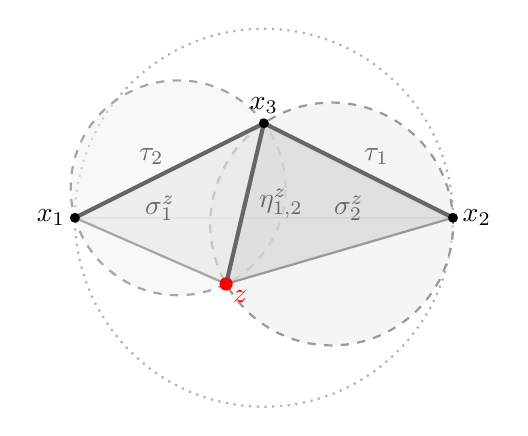
\begin{tikzpicture}[scale=1.2]
            % Coordonnées
            \coordinate (C) at (0,0);
            \coordinate (S) at (-2,0);
            \coordinate (T) at (2,0);
            \coordinate (U) at (0,1);
            \coordinate (Z) at (-0.4,-0.7);

            % Centres et rayons des nouvelles boules minimales
            % Par calcul exact géométrique des cercles circonscrits pour z = (-0.4, -0.7)
            \coordinate (Ct) at (-0.908, 0.317);
            \coordinate (Cs) at (0.717, -0.066);
            \def\Rt{1.137}
            \def\Rs{1.285}

            % Boule originale en filigrane (repère visuel)
            \draw[dotted, gray!60, thick] (C) circle (2);
            
            % L'arête non-active tau_u={s,t} est grisée pour montrer qu'elle n'est pas dans le chemin
            \draw[thick, gray!40] (S) -- (T);

            % Boules minimales des simplexes alternatifs
            \fill[gray!10, fill opacity=0.5] (Ct) circle (\Rt);
            \draw[dashed, gray!70, thick] (Ct) circle (\Rt);

            \fill[gray!15, fill opacity=0.5] (Cs) circle (\Rs);
            \draw[dashed, gray!80, thick] (Cs) circle (\Rs);

            % Simplexes alternatifs construits avec z
            \fill[gray!20, fill opacity=0.6] (S) -- (U) -- (Z) -- cycle;
            \draw[thick, gray!70] (S) -- (U) -- (Z) -- cycle;

            \fill[gray!35, fill opacity=0.6] (T) -- (U) -- (Z) -- cycle;
            \draw[thick, gray!80] (T) -- (U) -- (Z) -- cycle;

            % Chemin des facettes actives (en gras pour bien le faire ressortir)
            \draw[line width=1.5pt, gray!80!black] (S) -- (U) node[midway, above left=-2pt] {$\tau_2$};
            \draw[line width=1.5pt, gray!80!black] (T) -- (U) node[midway, above right=-2pt] {$\tau_1$};
            \draw[line width=1.5pt, gray!80!black] (U) -- (Z) node[midway, right=1pt] {$\eta_{1,2}^z$};

            % Sommets et intrus
            \fill (S) circle (1.5pt) node[left] {$x_1$};
            \fill (T) circle (1.5pt) node[right] {$x_2$};
            \fill (U) circle (1.5pt) node[above] {$x_3$};
            \fill[red] (Z) circle (2pt) node[below right=-1pt, red] {$z$};

            % Étiquettes des simplexes
            \node[gray!80!black] at (-1.1, 0.1) {$\sigma_1^z$};
            \node[gray!80!black] at (0.9, 0.1) {$\sigma_2^z$};
            
        \end{tikzpicture}
        \caption{Les $K$-simplexes $\sigma_2^z$ et $\sigma_1^z$ ont des rayons $ < r$. Le chemin $\tau_1 \xleftrightarrow{\sigma_1^z}_r \eta_{1,2}^z \xleftrightarrow{\sigma_2^z}_r \tau_2$ connecte les facettes actives dans $\Gamma_K(\mathcal{X})_{<r}$.}
        \label{fig:thm6_b}
    \end{subfigure}
    \caption{Illustration de la preuve du \Th~\ref{th:chapIV_separant_gabriel} ($K=2$) pour un triangle $\sigma=\{x_1,x_2,x_3\}$ obtus en $x_3$, c'est-à-dire que $S = \{x_1,x_2\}$. Si le simplexe n'est pas de \nom{Gabriel}, $B_\sigma$ (de rayon $r$) contient donc un ``intrus'' $z$. Les facettes $\tau_1$ et $\tau_2$, actives pour une filtration $<r$, sont connectées au moyen de $z$ (les $2$-simplexes $\sigma_s^z$ et $\sigma_t^z$).}
    \label{fig:preuve_gabriel_obtus}
\end{figure}


D'après la définition d'un simplexe $K$-séparant (\Def[def:chapIV_simplexe_separant]) et la remarque associée, les facettes actives de $\sigma$ (c'est-à-dire celles existant strictement avant $r$) sont exactement les facettes
\[
    \tau_s\eqdef\sigma\setminus\{s\},
    \qquad s\in S.
\]

Montrons maintenant que toutes les facettes actives $\tau_s$, $s\in S$, sont déjà dans la même composante de $\Gamma_K(\mathcal X)_{<r}$.
Soient $s,t\in S$, $s\neq t$. Considérons les deux $K$-simplexes
\[
    \sigma_s^z\eqdef(\sigma\setminus\{s\})\cup\{z\},
    \qquad
    \sigma_t^z\eqdef(\sigma\setminus\{t\})\cup\{z\}.
\]
Ils contiennent respectivement les facettes
\[
    \tau_s=\sigma\setminus\{s\},
    \qquad
    \eta_{s,t}^z\eqdef(\sigma\setminus\{s,t\})\cup\{z\},
\]
et
\[
    \eta_{s,t}^z,
    \qquad
    \tau_t=\sigma\setminus\{t\}.
\]
Il suffit donc de vérifier que
\[
    \rho(\sigma_s^z)<r
    \qquad\text{et}\qquad
    \rho(\sigma_t^z)<r.
\]
(Voir la \Fig~\ref{fig:preuve_gabriel_obtus} pour une illustration.)
Or $\sigma_s^z$ est contenu dans $B_\sigma$, et ses points situés sur la frontière de $B_\sigma$ sont contenus dans $S\setminus\{s\}$. D'après le \Res~\ref{res:chapIV_miniball_support}, on a bien
\[
\rho(\sigma_s^z)<r.
\]
Même raisonnement pour $\sigma_t^z$.

Ainsi, pour tout couple $s,t\in S$, les facettes $\tau_s$ et $\tau_t$ sont reliées dans $ \Gamma_K(\mathcal X)_{<r}$ par le chemin
\[
    \tau_s \xleftrightarrow{\sigma_s^z}_r \eta_{s,t}^z \xleftrightarrow{\sigma_t^z}_r \tau_t
\]
Le simplexe $\sigma$ n'a donc aucune influence sur les $K$-polyèdres (les $(K-1)$-simplexes déjà existants étant de la même composante connexe ; ceux apparaissant ayant déjà tous leurs points dans cette même composante préexistante) ; il n'est pas $K$-séparant.
\end{Preuve}

\begin{Definition}{$K$-graphe de \nom{Gabriel}}{chapIV_graphe_k_gabriel}
Le $K$-\emph{graphe de \nom{Gabriel}} de $\mathcal X$, noté
\[
\boxed{
    \mathcal G_K^{\mathrm{Gab}}(\mathcal X),
    }
\]
est le sous-graphe pondéré de $\Gamma_K(\mathcal X)$ défini ainsi.
\begin{itemize}
    \item Ses sommets sont les $(K-1)$-simplexes de $\mathcal X$ qui sont facettes d'au moins un $K$-simplexe de \nom{Gabriel}.
    \item Pour chaque $K$-simplexe de \nom{Gabriel} $\sigma$, on relie entre elles toutes les facettes de $\sigma$ (formant une clique).
    \item Toutes les arêtes induites par $\sigma$ reçoivent le poids $\rho(\sigma)$.
\end{itemize}
\end{Definition}

Pour $K=1$, ce graphe n'est autre que le graphe de \nom{Gabriel} classique, pondéré par la moitié de la longueur des arêtes. Pour $K\ge2$, ce n'est plus un graphe sur les points, mais un graphe sur les $(K-1)$-simplexes. %C'est exactement ce qu'il faut : les objets qui percolent ne sont plus les points, mais les facettes.

\begin{Fait}{Le graphe de \nom{Gabriel} contient toutes les fusions utiles}{chapIV_gabriel_preserve_fusions}
Pour tout $r\ge0$, les ensembles de points associés aux composantes connexes non réduites à un sommet isolé de
\[
    \mathcal G_K^{\mathrm{Gab}}(\mathcal X)_{\le r}
\]
coïncident avec les $K$-polyèdres de $\check C(\mathcal X,r)$ non réduits à un $(K-1)$-simplexe isolé.
\end{Fait}

\begin{Preuve}
Notons d'abord l'inclusion triviale
\[
    \mathcal G_K^{\mathrm{Gab}}(\mathcal X)_{\le r}
    \subseteq
    \Gamma_K(\mathcal X)_{\le r}.
\]
% est immédiate : (tout simplexe \nom{Gabriel} de poids au plus $r$ appartient au complexe de \v Cech au rayon $r$.
Supposons (preuve par induction avec rayon $r$ croissant) que jusqu'à un niveau critique $r$, les composantes non triviales (vues comme des ensembles de points) du graphe de \nom{Gabriel} et du graphe de \v Cech des facettes définissent les mêmes ensembles de points. Ajoutons maintenant les $K$-simplexes de naissance $r$.

Si un simplexe $\sigma$ ajouté à ce niveau est de \nom{Gabriel}, il est ajouté dans les deux graphes. S'il ne l'est pas, la preuve du \Th~\ref{th:chapIV_separant_gabriel} montre que toutes ses facettes nées strictement avant $r$ sont déjà reliées entre elles par des chemins de poids strictement plus petits que $r$. %\textcolor{red}{Revoir la preuve.} 
Les autres facettes de $\sigma$ naissent au niveau $r$ lui-même ; elles peuvent être ajoutées comme sommets, mais elles ne changent pas l'ensemble de points de la composante, car l'union des facettes actives
\[
    \{\sigma\setminus\{s\}\, \mid \, s\in\sigma\cap\partial B_\sigma\}
\]
contient déjà tous les sommets de $\sigma$. Ajouter $\sigma$ ne crée donc aucune fusion nouvelle entre ensembles de points.

Par induction sur les valeurs critiques, les simplexes qui ne sont pas de \nom{Gabriel} peuvent être supprimés sans modifier les $K$-polyèdres non triviaux.
\end{Preuve}

Nous pouvons maintenant définir l'analogue de l'arbre minimum couvrant.

\begin{Definition}{$K$-arbre minimum couvrant}{chapIV_kmst}
Un \emph{$K$-arbre minimum couvrant}, noté $K\text{-}\mathrm{MST}$, est un arbre minimum couvrant du graphe pondéré $\mathcal G_K^{\mathrm{Gab}}(\mathcal X)$.
Pour $r\ge0$, on note
\[
\boxed{
    K\text{-}\mathrm{MST}_{\le r}
    }
\]
le sous-graphe obtenu en supprimant les arêtes de poids strictement supérieur à $r$.
\end{Definition}


\begin{Theoreme}{Complexe de \v Cech $\equiv$ $K$-arbre minimum couvrant élagué}{chapIV_cech_kmst}
Supposons $\mathcal X\subset\mathbb R^p$ en position générale pour la filtration de \v Cech. Pour tout $r\ge0$, les ensembles de points associés aux composantes connexes de
\[
    K\text{-}\mathrm{MST}_{\le r}
\]
qui ne sont pas réduites à un sommet isolé coïncident avec les $K$-polyèdres de $\check C(\mathcal X,r)$ qui ne sont pas réduits à un $(K-1)$-simplexe isolé.
\end{Theoreme}

\begin{Preuve}[{Preuve du \Th~\ref{th:chapIV_cech_kmst}}]
On applique le \Res~\ref{res:chapIV_mst_sous_niveaux_graphe} au graphe pondéré
\[
    \mathcal G_K^{\mathrm{Gab}}(\mathcal X).
\]
Il donne, pour tout $r\ge0$, l'égalité des composantes connexes de
\[
    K\text{-}\mathrm{MST}_{\le r}
    \qquad\text{et}\qquad
    \mathcal G_K^{\mathrm{Gab}}(\mathcal X)_{\le r}.
\]
Le \Fact~\ref{fait:chapIV_gabriel_preserve_fusions} identifie ensuite les composantes non triviales de ce dernier graphe avec les $K$-polyèdres non triviaux de $\check C(\mathcal X,r)$.
\end{Preuve}

% \Remarque{Les $(K-1)$-simplexes isolés ne sont pas perdus mathématiquement : leur naissance est simplement donnée par leur rayon $\rho(\tau)$. Le $K$-MST encode les fusions, pas la liste complète de tous les simplexes isolés. Pour reconstruire strictement toute la hiérarchie, il suffit donc de stocker en plus les naissances des $(K-1)$-simplexes que l'on souhaite faire apparaître comme clusters élémentaires.}

\section{La bonne structure à observer : la mosaïque de \nom{Delaunay} d'ordre $K$}
\label{sec:chapIV_delaunay_ordre_k}

Le \Th~\ref{th:chapIV_cech_kmst} remplace le complexe de \v Cech complet par un arbre couvrant construit sur le $K$-graphe de \nom{Gabriel}. Il reste encore à savoir : comment trouver les simplexes de \nom{Gabriel} sans tester les $\binom n{K+1}$ candidats ?

Pour $K=1$, la réponse dans l'espace euclidien $\mathbb R^p$ est la triangulation de \nom{Delaunay} (\Res~\ref{res:MSTsous-graphe}). 

Pour $K\ge2$, la réponse est la mosaïque de \nom{Delaunay} d'ordre $K$ \cite{edelsbrunnerOsang2021multicover, osangEdelsbrunner2023algorithm}.
(Pour la dimension $p=2$, voir en particulier \cite{MitscheSaumellSilveira2011HigherOrderDelaunay}.)



\begin{Definition}{Cellules de \nom{Voronoï} d'ordre supérieur et mosaïque de \nom{Delaunay} duale \cite{edelsbrunnerOsang2021multicover, osangEdelsbrunner2023algorithm}}{mosaïque_delaunay_ordre_k}
Soit $\mathcal X \subseteq \mathbb R^p$ un ensemble fini, et soit $k \in \{1,\ldots,|\mathcal X|-1\}$.
Pour tout sous-ensemble $Q \subset \mathcal X$ de cardinal $k$, on définit sa cellule de \nom{Voronoï} d'ordre $k$ par
\[
    \operatorname{Vor}_k(Q)
    \eqdef
    \left\{
        y \in \mathbb R^p
        \ \middle|\
        \max_{q\in Q} \norme{y-q}
        \le
        \min_{x\in \mathcal X\setminus Q} \norme{y-x}
    \right\}.
\]
Autrement dit, $\operatorname{Vor}_k(Q)$ est l'ensemble des points de l'espace pour lesquels les points de $Q$ sont les $k$ plus proches voisins dans $\mathcal X$.

La \emph{mosaïque de \nom{Delaunay} d'ordre $k$}, notée $\operatorname{Del}_k(\mathcal X)$, est le complexe dual du diagramme de \nom{Voronoï} d'ordre $k$ : ses sommets sont les $k$-uplets $Q \subset \mathcal X$ tels que $\operatorname{Vor}_k(Q)\neq\emptyset$, et plus généralement
\[
    \{Q_0,\ldots,Q_m\} \in \operatorname{Del}_k(\mathcal X)
    \quad\Longleftrightarrow\quad
    \bigcap_{i=0}^m \operatorname{Vor}_k(Q_i) \neq \emptyset.
\]
En particulier, deux sommets $Q,Q'$ de $\operatorname{Del}_k(\mathcal X)$ sont adjacents dès qu'il existe un point $y\in\mathbb R^p$ pour lequel $Q$ et $Q'$ sont deux choix possibles de $k$ plus proches voisins.

Nous dirons qu'un $k$-simplexe $\sigma\subset\mathcal X$ est \emph{porté par la mosaïque de \nom{Delaunay} d'ordre $k$} s'il existe deux sommets adjacents $Q,Q'$ de $\operatorname{Del}_k(\mathcal X)$ tels que
\[
    Q\cup Q'=\sigma.
\]
%Cette convention identifie donc un $K$-simplexe à un échange élémentaire entre deux listes de $K$ plus proches voisins.
\end{Definition}

\subsection{Un $K$-simplexe de \nom{Gabriel} est nécessairement dans la mosaïque de \nom{Delaunay} d'ordre $K$}

\begin{Theoreme}{Les $K$-simplexes de \nom{Gabriel} sont portés par la mosaïque de \nom{Delaunay} d'ordre $K$}{gabriel_dans_mosaique_ordre_k}
Soit $\mathcal X\subset\mathbb R^p$ un nuage fini en position générale.
Tout $K$-simplexe de \nom{Gabriel} $\sigma\subseteq\mathcal X$ est porté par la mosaïque de \nom{Delaunay} d'ordre $K$, au sens de la \Def~\ref{def:mosaïque_delaunay_ordre_k}.
\end{Theoreme}

\begin{Preuve}[Preuve du \Th~\ref{th:gabriel_dans_mosaique_ordre_k}] 
Notons
\[
    B_\sigma=\overline B(c_\sigma,r_\sigma)
\]
la plus petite boule fermée contenant $\sigma$.
Comme $\sigma$ est de \nom{Gabriel}, aucun point de $\mathcal X\setminus\sigma$ n'appartient à l'intérieur de cette boule :
\[
    \mathring B_\sigma\cap(\mathcal X\setminus\sigma)=\varnothing.
\]
En position générale, on peut de plus supposer qu'aucun point de $\mathcal X\setminus\sigma$ n'appartient à la sphère $\partial B_\sigma$.
L'on décompose alors les sommets de $\sigma$ en deux familles :
\[
    I \eqdef \sigma\cap \mathring B_\sigma,
    \qquad
    S \eqdef \sigma\cap \partial  B_\sigma.
\]
Les points de $I$ sont strictement plus proches du centre $c_\sigma$ que les points de $S$, tandis que tous les points de $S$ sont à distance exactement $r_\sigma$ de $c_\sigma$.
La boule $B_\sigma$ étant minimale, l'ensemble $S$ contient au moins deux points. Choisissons donc deux sommets distincts $s,t\in S$.
Considérons les deux $K$-uplets
\[
    Q_s \eqdef \sigma\setminus\{s\},
    \qquad
    Q_t \eqdef \sigma\setminus\{t\}.
\]
Au point $c_\sigma$, tous les points de $I$ sont strictement plus proches que les points de $S$, et aucun point extérieur à $\sigma$ n'est plus proche que les points de $S$.
Ainsi, $Q_s$ et $Q_t$ sont deux choix possibles de $K$ plus proches voisins de $c_\sigma$.
Autrement dit,
\[
    c_\sigma\in \operatorname{Vor}_K(Q_s)\cap \operatorname{Vor}_K(Q_t).
\]
Par définition de la mosaïque de \nom{Delaunay} d'ordre $K$, les deux sommets $Q_s$ et $Q_t$ sont donc adjacents dans $\operatorname{Del}_K(\mathcal X)$.
Enfin,
\[
    Q_s\cup Q_t
    =
    (\sigma\setminus\{s\})\cup(\sigma\setminus\{t\})
    =
    \sigma,
\]
ce qui prouve que $\sigma$ est porté par la mosaïque de \nom{Delaunay} d'ordre $K$.
\end{Preuve}

%\textcolor{red}{Proposer un algorithme ?}

% \begin{algorithm}[H]
% \caption{Construction exacte de la hiérarchie depuis la mosaïque de \nom{Delaunay} d'ordre $K$}
% \label{alg:hierarchie_mosaique_delaunay_k}
% \begin{algorithmic}[1]
% \Require Nuage fini $\mathcal X\subset\mathbb R^p$, entier $K\ge 1$
% \Ensure Hiérarchie des $K$-polyèdres de la filtration de \v Cech

% \State Construire la mosaïque de \nom{Delaunay} d'ordre $K$, $\operatorname{Del}_K(\mathcal X)$.
% \State Initialiser une famille vide $\mathcal S_K$ de $K$-simplexes pondérés.

% \For{chaque arête $(Q,Q')$ du $1$-squelette de $\operatorname{Del}_K(\mathcal X)$}
%     \State $\sigma \gets Q\cup Q'$
%     \If{$|\sigma|=K+1$}
%         \State Calculer la plus petite boule englobante $B_{\min}(\sigma)$ et son rayon $r(\sigma)$.
%         \If{$\mathring B_{\min}(\sigma)\cap(\mathcal X\setminus\sigma)=\emptyset$}
%             \State Ajouter $\sigma$ à $\mathcal S_K$ avec poids $r(\sigma)$.
%         \EndIf
%     \EndIf
% \EndFor

% \State Construire le graphe auxiliaire $G_K$ :
% \Statex \hspace{\algorithmicindent} ses sommets sont les $(K-1)$-faces des simplexes de $\mathcal S_K$ ;
% \Statex \hspace{\algorithmicindent} pour chaque $\sigma\in\mathcal S_K$, relier toutes les $(K-1)$-faces de $\sigma$ avec le poids $r(\sigma)$.

% \State Appliquer l'algorithme de \nom{Kruskal} à $G_K$.
% \State Enregistrer, par ordre croissant des poids, les fusions de composantes connexes.
% \State \Return La hiérarchie obtenue.

% \end{algorithmic}
% \end{algorithm}


% L'algorithme précédent est simplement la version géométrique de l'algorithme de \nom{Kruskal}.
% La mosaïque de \nom{Delaunay} d'ordre $K$ fournit l'ensemble des échanges possibles entre $K$ plus proches voisins.
% Le \Th~\ref{th:gabriel_dans_mosaique_ordre_k} garantit que tous les simplexes $K$-\nom{Gabriel}, donc en particulier tous les simplexes $K$-séparants, apparaissent parmi ces échanges.
% Il suffit alors de filtrer ces candidats par la condition de vacuité $K$-\nom{Gabriel}, puis de construire le graphe auxiliaire sur les $(K-1)$-faces.
% Les composantes connexes de ce graphe, lorsqu'on ne conserve que les arêtes de poids au plus $r$, coïncident avec les $K$-polyèdres de $\check C(\mathcal X,r)$.
% Ainsi, la hiérarchie complète est obtenue sans jamais énumérer les $\binom{|\mathcal X|}{K+1}$ simplexes du complexe de \v Cech complet.














% \subsection*{Le cas favorable de la connexité par triangles : $K=2$}

% Pour $K=2$, les sommets du graphe $2$-\nom{Gabriel} sont des arêtes de $\mathcal X$, et ses arêtes sont induites par des triangles $2$-\nom{Gabriel}. En dimension $2$, on peut les extraire à partir de la triangulation de \nom{Delaunay} ordinaire.

% \begin{Fait}{Triangles $2$-\nom{Gabriel} et triangulation de \nom{Delaunay} planaire \cite{BibiAppliedNetworkScience}}{chapIV_2gabriel_delaunay}
% Supposons $\mathcal X\subset\mathbb R^2$ en position générale.
% Soit $\sigma=\{a,b,c\}$ un triangle $2$-\nom{Gabriel}.
% \begin{enumerate}
%     \item Si $\sigma$ est acutangle, alors $\sigma$ est une face de la triangulation de \nom{Delaunay} ordinaire.
%     \item Si $\sigma$ est obtusangle en $a$, de plus long côté $[b,c]$, alors les deux arêtes courtes $[a,b]$ et $[a,c]$ sont des arêtes de la triangulation de \nom{Delaunay} ordinaire.
% \end{enumerate}
% \end{Fait}

% \begin{Preuve}
% Si le triangle est acutangle, sa plus petite boule englobante est son disque circonscrit. Comme le triangle est $2$-\nom{Gabriel}, ce disque ne contient aucun autre point de $\mathcal X$ dans son intérieur. C'est exactement le critère du cercle vide pour être une face de \nom{Delaunay} dans le plan.

% Supposons maintenant que le triangle soit obtusangle en $a$. Sa plus petite boule englobante est le disque $D$ de diamètre $[b,c]$, et $a$ appartient à l'intérieur de $D$. La condition $2$-\nom{Gabriel} dit que $D$ ne contient aucun point de $\mathcal X\setminus\{a,b,c\}$ dans son intérieur.

% Montrons que $[a,b]$ est une arête de \nom{Delaunay}. Comme $a$ est à l'intérieur de $D$ et $b$ sur $\partial D$, il existe un disque $D_b$ contenu dans $D$, tangent intérieurement à $D$ au point $b$, et dont la frontière passe par $a$ et $b$. Son intérieur est inclus dans celui de $D$, et il ne contient donc aucun point de $\mathcal X\setminus\{a,b,c\}$. Le point $c$, distinct de $b$, appartient à $\partial D$ et n'appartient pas à l'intérieur de $D_b$. Le disque $D_b$ est donc un disque vide passant par $a$ et $b$, ce qui prouve que $[a,b]$ est une arête de \nom{Delaunay}. Le même argument au point $c$ montre que $[a,c]$ est une arête de \nom{Delaunay}.
% \end{Preuve}

% Le \Fact~\ref{fait:chapIV_2gabriel_delaunay} donne une procédure d'extraction. Elle est écrite ci-dessous dans sa version conceptuelle ; une implémentation efficace utilise une structure de requêtes de plus proches voisins ou de recherche dans les boules.

% \begin{algorithm}[H]
% \caption{Extraction du graphe $2$-\nom{Gabriel} dans le plan}
% \label{alg:chapIV_extraction_2gabriel}
% \begin{algorithmic}[1]
% \Require Nuage $\mathcal X\subset\mathbb R^2$ en position générale
% \Ensure Graphe pondéré $\mathcal G^{\mathrm{Gab}}_2(\mathcal X)$
% \State $\mathcal D\gets\nom{TriangulationDelaunay}(\mathcal X)$
% \State Initialiser $\mathcal G\gets\varnothing$
% \Statex
% \State \Comment{Triangles acutangles : faces de \nom{Delaunay}}
% \ForAll{faces triangulaires $\{a,b,c\}$ de $\mathcal D$}
%     \State Calculer la plus petite boule englobante $B_\sigma=\overline B(c_\sigma,\rho(\sigma))$ de $\sigma=\{a,b,c\}$
%     \If{$B_\sigma$ est le disque circonscrit de $\sigma$}
%         \State Ajouter les sommets $\{a,b\}$, $\{a,c\}$, $\{b,c\}$ à $\mathcal G$
%         \State Ajouter la clique entre ces trois sommets, de poids $\rho(\sigma)$
%     \EndIf
% \EndFor
% \Statex
% \State \Comment{Triangles obtus : deux côtés courts sont des arêtes de \nom{Delaunay}}
% \ForAll{$a\in\mathcal X$}
%     \ForAll{paires distinctes $b,c$ de voisins de $a$ dans le graphe de \nom{Delaunay} $\mathcal D$}
%         \State $m\gets (b+c)/2$ et $r\gets \norme{b-c}/2$
%         \If{$\norme{a-m}<r$ \textbf{et} $B(m,r)^\circ\cap(\mathcal X\setminus\{a,b,c\})=\varnothing$}
%             \State $\sigma\gets\{a,b,c\}$
%             \State Ajouter les sommets $\{a,b\}$, $\{a,c\}$, $\{b,c\}$ à $\mathcal G$
%             \State Ajouter la clique entre ces trois sommets, de poids $r$
%         \EndIf
%     \EndFor
% \EndFor
% \State \Return $\mathcal G$
% \end{algorithmic}
% \end{algorithm}

% La première boucle parcourt un nombre linéaire de faces en dimension $2$ lorsque le nuage est en position générale : la triangulation de \nom{Delaunay} planaire a $\mathcal O(n)$ arêtes et faces, et se calcule en $\mathcal O(n\log n)$ \cite{Delaunay2D, BoissonnatChazalYvinec}. La seconde boucle est celle qui demande le plus de soin en pratique. Écrite naïvement, elle parcourt les paires de voisins de \nom{Delaunay} autour de chaque sommet ; sur des nuages non pathologiques, cela reste quasi linéaire, mais le pire cas combinatoire impose d'utiliser un balayage angulaire ou une structure de requêtes géométriques pour conserver une complexité raisonnable.

% Une fois $\mathcal G^{\mathrm{Gab}}_2(\mathcal X)$ construit, l'algorithme final est exactement celui que l'on espérait : on calcule une forêt couvrante minimum de ce graphe, puis on l'élague au rayon désiré. D'après le \Th~\ref{th:chapIV_cech_kmst}, on obtient alors les mêmes $2$-polyèdres non triviaux que ceux du complexe de \v Cech complet, mais sans construire tous les triangles possibles.

Nous avons à présent tous les résultats nécessaires pour aborder dès le chapitre suivant les aspects pratiques.

\Synthese{Le rôle de l'arbre minimum couvrant dans le Single-Linkage repose sur un principe plus général : dans une filtration, seules les cellules qui changent effectivement la connectivité doivent être conservées pour reconstruire les composantes à toutes les échelles.

Pour les $K$-polyèdres, ces cellules sont les simplexes $K$-séparants. Le \Th~\ref{th:chapIV_separant_gabriel} montre qu'ils satisfont nécessairement une condition de vacuité : ils sont de \nom{Gabriel}. 
On peut donc remplacer le graphe complet des facettes de \v Cech par le graphe beaucoup plus mince des simplexes de \nom{Gabriel}, puis calculer un $K$-arbre minimum couvrant. L'élagage de cet arbre redonne exactement les mêmes $K$-polyèdres non triviaux que la hiérarchie complète sur le complexe de \v Cech (\Th~\ref{th:chapIV_cech_kmst}).

La structure géométrique qui organise ces simplexes est la mosaïque de \nom{Delaunay} d'ordre $K$ (\Th~\ref{th:gabriel_dans_mosaique_ordre_k}).}
